\usepackage{../pvm}

\usetikzlibrary{arrows.meta}

\title{Inheritance}
\author{Fr\'ed\'eric Vogels}


\begin{document}

\begin{frame}
  \titlepage
\end{frame}

\begin{frame}
  \frametitle{Inheritance}
  \structure{Key differences from Java}
  \begin{itemize}
    \item Meaning of protected
    \item Public/protected/private inheritance
    \item Virtual methods
    \item Multiple inheritance
    \item No interfaces
  \end{itemize}
\end{frame}

\section{{\tt protected}}

\begin{frame}
  \tableofcontents[currentsection]
\end{frame}

\begin{frame}
  \frametitle{{\tt protected} in Java}
  \structure{Who can reach a {\tt protected} member?}
  \begin{itemize}
    \item Objects of the same class
    \item Objects of a class from the same package
    \item Objects of a subclass
  \end{itemize}
  \vskip5mm
  \structure{Who cannot reach a {\tt protected} member?}
  \begin{itemize}
    \item Objects of a class not in the same package and not a subclass
  \end{itemize}
\end{frame}

\begin{frame}
  \frametitle{{\tt protected} in \cpp}
  \structure{Who can reach a {\tt protected} member?}
  \begin{itemize}
    \item Objects of the same class
    \item Objects of a subclass
  \end{itemize}
  \vskip5mm
  \structure{Who cannot reach a {\tt protected} member?}
  \begin{itemize}
    \item Objects of a class that is not a subclass
  \end{itemize}
\end{frame}

\section{Types of inheritance}

\begin{frame}
  \tableofcontents[currentsection]
\end{frame}

\begin{frame}
  \frametitle{Types of Inheritance}
  \structure{Java}
  \begin{itemize}
    \item Public inheritance
  \end{itemize}
  \vskip5mm
  \structure{\cpp}
  \begin{itemize}
    \item Public inheritance
    \item Protected inheritance
    \item Private inheritance
  \end{itemize}
\end{frame}

\begin{frame}
  \frametitle{Inheritance in Java}
  \begin{center}
    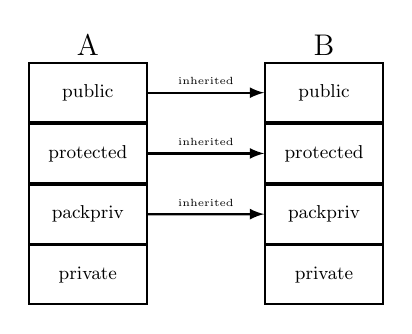
\begin{tikzpicture}[part/.style={draw,thick,minimum width=2cm,minimum height=1cm,font=\small},
                        inheritance/.style={-latex,thick},
                        scale=.75,transform shape]
      \node[part] (A public) at (0,0) {public};
      \node[part,anchor=north west] (A protected) at (A public.south west) {protected};
      \node[part,anchor=north west] (A package) at (A protected.south west) {packpriv};
      \node[part,anchor=north west] (A private) at (A package.south west) {private};
      \node[anchor=south,font=\Large] at (A public.north) {A};

      \node[part] (B public) at (4,0) {public};
      \node[part,anchor=north west] (B protected) at (B public.south west) {protected};
      \node[part,anchor=north west] (B package) at (B protected.south west) {packpriv};
      \node[part,anchor=north west] (B private) at (B package.south west) {private};
      \node[anchor=south,font=\Large] at (B public.north) {B};

      \draw[inheritance] (A public) -- (B public) node[midway,above,font=\tiny] {inherited};
      \draw[inheritance] (A protected) -- (B protected) node[midway,above,font=\tiny] {inherited};
      \draw[inheritance] (A package) -- (B package) node[midway,above,font=\tiny] {inherited};
    \end{tikzpicture}
  \end{center}
  \structure{When {\tt B} inherits from {\tt A}\dots}
  \begin{itemize}
    \item {\tt A}'s public members $\rightarrow$ {\tt B}'s public members
    \item {\tt A}'s protected members $\rightarrow$ {\tt B}'s protected members
    \item {\tt A}'s package private members $\rightarrow$ {\tt B}'s package private
    \item {\tt A}'s private members are not inherited \\ (half-lie, but you know what I mean)
  \end{itemize}
\end{frame}

\begin{frame}
  \frametitle{Public Inheritance in \cpp}
  \begin{center}
    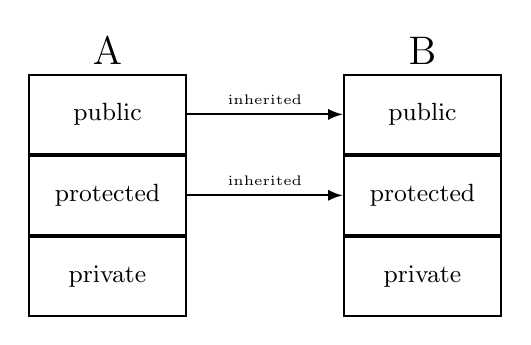
\begin{tikzpicture}[part/.style={draw,thick,minimum width=2cm,minimum height=1cm,font=\small},
                        inheritance/.style={-latex,thick}]
      \node[part] (A public) at (0,0) {public};
      \node[part,anchor=north west] (A protected) at (A public.south west) {protected};
      \node[part,anchor=north west] (A private) at (A protected.south west) {private};
      \node[anchor=south,font=\Large] at (A public.north) {A};

      \node[part] (B public) at (4,0) {public};
      \node[part,anchor=north west] (B protected) at (B public.south west) {protected};
      \node[part,anchor=north west] (B private) at (B protected.south west) {private};
      \node[anchor=south,font=\Large] at (B public.north) {B};

      \draw[inheritance] (A public) -- (B public) node[midway,above,font=\tiny] {inherited};
      \draw[inheritance] (A protected) -- (B protected) node[midway,above,font=\tiny] {inherited};
    \end{tikzpicture}
  \end{center}
  \structure{Syntax}
  \code{public-inheritance-syntax.cpp}
\end{frame}

\begin{frame}
  \frametitle{Protected Inheritance in \cpp}
  \begin{center}
    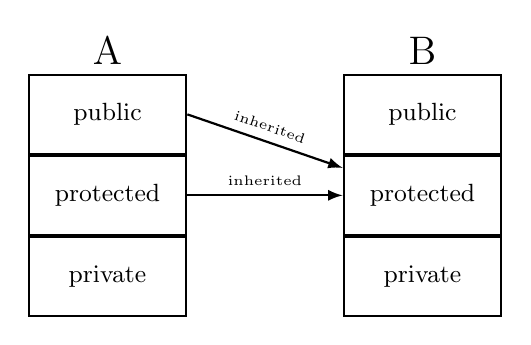
\begin{tikzpicture}[part/.style={draw,thick,minimum width=2cm,minimum height=1cm,font=\small},
                        inheritance/.style={-latex,thick}]
      \node[part] (A public) at (0,0) {public};
      \node[part,anchor=north west] (A protected) at (A public.south west) {protected};
      \node[part,anchor=north west] (A private) at (A protected.south west) {private};
      \node[anchor=south,font=\Large] at (A public.north) {A};

      \node[part] (B public) at (4,0) {public};
      \node[part,anchor=north west] (B protected) at (B public.south west) {protected};
      \node[part,anchor=north west] (B private) at (B protected.south west) {private};
      \node[anchor=south,font=\Large] at (B public.north) {B};

      \draw[inheritance] (A public.east) -- (B protected) node[midway,above,font=\tiny,sloped] {inherited};
      \draw[inheritance] (A protected) -- (B protected) node[midway,above,font=\tiny] {inherited};
    \end{tikzpicture}
  \end{center}
  \structure{Syntax}
  \code{protected-inheritance-syntax.cpp}
\end{frame}

\begin{frame}
  \frametitle{Private Inheritance in \cpp}
  \begin{center}
    \begin{tikzpicture}[part/.style={draw,thick,minimum width=2cm,minimum height=1cm,font=\small},
                        inheritance/.style={-latex,thick}]
      \node[part] (A public) at (0,0) {public};
      \node[part,anchor=north west] (A protected) at (A public.south west) {protected};
      \node[part,anchor=north west] (A private) at (A protected.south west) {private};
      \node[anchor=south,font=\Large] at (A public.north) {A};

      \node[part] (B public) at (4,0) {public};
      \node[part,anchor=north west] (B protected) at (B public.south west) {protected};
      \node[part,anchor=north west] (B private) at (B protected.south west) {private};
      \node[anchor=south,font=\Large] at (B public.north) {B};

      \draw[inheritance] (A public.east) -- ($ (B private.west) ! 0.25 ! (B private.north west) $) node[midway,above,font=\tiny,sloped] {inherited};
      \draw[inheritance] (A protected.east) -- ($ (B private.west) ! 0.25 ! (B private.south west) $) node[midway,above,font=\tiny,sloped] {inherited};
    \end{tikzpicture}
  \end{center}
  \structure{Syntax}
  \code{private-inheritance-syntax.cpp}
\end{frame}

\begin{frame}
  \frametitle{Public Inheritance: Example}
  \code[font size=\small]{public-inheritance.cpp}
\end{frame}

\begin{frame}
  \frametitle{Private Inheritance: Example}
  \code[font size=\small]{private-inheritance.cpp}
\end{frame}

\begin{frame}
  \frametitle{Liskov Violated?}
  \begin{overprint}
    \onslide<handout:0|1>
    \begin{center}
      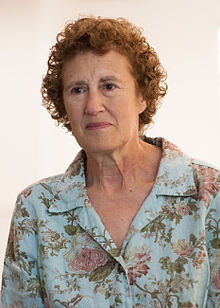
\includegraphics[width=3cm]{sad-liskov.jpg} \\
      \tiny (saddest picture I could find)
    \end{center}
    \onslide<handout:0|2>
    \begin{center}
      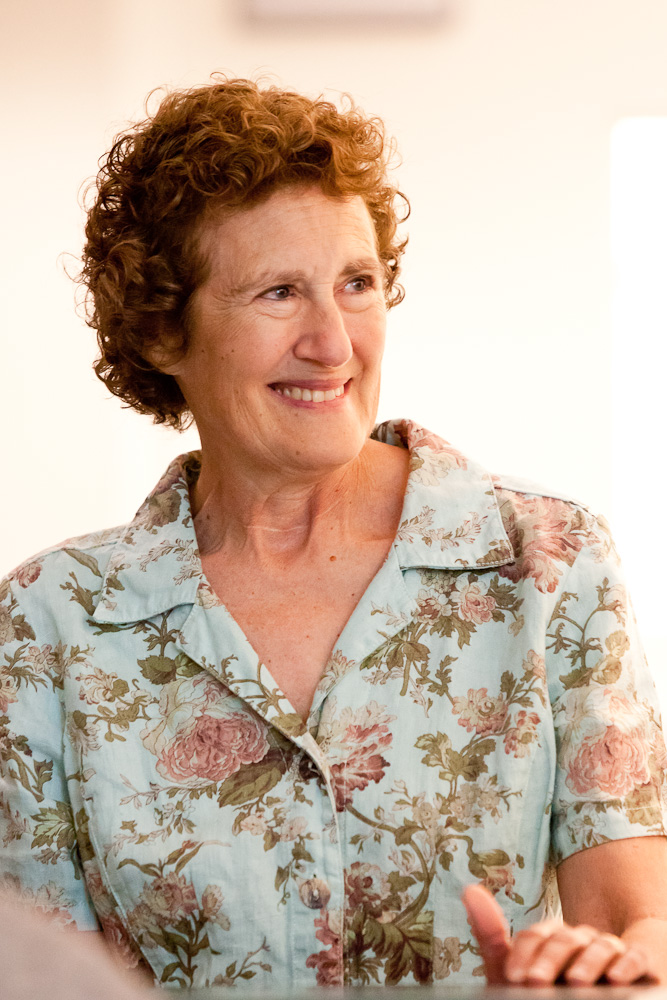
\includegraphics[width=3cm]{happy-liskov.jpg} \\
      \tiny (happiest picture I could find)
    \end{center}
  \end{overprint}
  \vskip5mm
  \begin{overprint}
    \onslide<handout:1|1>
    \begin{itemize}
      \item Protected and private inheritance seemingly violate LSP
      \item Superclass has public member {\tt X}
      \item Then every subclass should also have public member {\tt X}
      \item Not the case with protected/private inheritance
    \end{itemize}

    \onslide<handout:2|2>
    \begin{itemize}
      \item Liskov not actually violated!
      \item Subtype relation has also changed!
    \end{itemize}
  \end{overprint}
\end{frame}

\begin{frame}
  \frametitle{Subtype Relation In Java}
  \begin{itemize}
    \item Given class {\tt A}
    \item Given class {\tt B}, subclass of {\tt A}
    \item {\tt B} is then a \emph{subtype} of {\tt A}
    \item Everywhere an {\tt A} is needed, a {\tt B} will work too
  \end{itemize}
  \code[font size=\small,language=java]{subtype.java}
\end{frame}

\begin{frame}
  \frametitle{Subtype Relation In \cpp}
  \begin{itemize}
    \item Public inheritance: {\tt B} is a subtype of {\tt A}
    \item Nonpublic inheritance: {\tt B} is \emph{not} a subtype of {\tt A}
  \end{itemize}
  \code[font size=\small]{subtype.cpp}
\end{frame}

\section{Virtual Methods}

\begin{frame}
  \tableofcontents[currentsection]
\end{frame}

\begin{frame}
  \frametitle{Virtual Methods}
  \begin{itemize}
    \item Virtual methods: methods that are overridable
    \item When calling a virtual method, dynamic type determines which version is called
    \item When calling a nonvirtual method, static type determines which version is called
    \item In Java, all (nonprivate) object methods are virtual
  \end{itemize}
\end{frame}

\begin{frame}
  \frametitle{Virtual Methods in \cpp}
  \begin{itemize}
    \item If you want a member function to be overridable, you have to be explicit about it
    \item To make virtual: add {\tt virtual}
    \item To override: add {\tt override} (optional, but encouraged)
  \end{itemize}
  \vskip5mm
  \structure{Syntax}
  \code{virtual-syntax.cpp}
\end{frame}

\begin{frame}
  \frametitle{Example}
  \code{virtual-example1.cpp}
\end{frame}

\begin{frame}
  \frametitle{Example}
  \code{virtual-example2.cpp}
\end{frame}

\begin{frame}
  \frametitle{Inheritance in \cpp}
  \begin{itemize}
    \item When working with inheritance, always use pointers/references
    \item When working by-value, inheritance won't work correctly
    \item Why would that be? \cake
  \end{itemize}
  \code{inheritance-by-value.cpp}
\end{frame}

\begin{frame}
  \frametitle{Abstract Methods}
  \begin{itemize}
    \item Abstract method = virtual method without body
    \item In Java: use {\tt abstract}
    \item \cpp\ has no {\tt abstract} keyword
    \item To declare abstract method: {\tt = 0}
  \end{itemize}
  \structure{Syntax}
  \code{abstract-syntax.cpp}
\end{frame}

\begin{frame}
  \frametitle{Abstract Classes}
  \begin{itemize}
    \item Java: requires to add {\tt abstract} to class
    \item \cpp: class is automatically abstract when it contains 1+ abstract methods
    \item Abstract classes cannot be instantiated
  \end{itemize}
\end{frame}

\begin{frame}
  \frametitle{Example}
  \code[font size=\small]{abstract-example.cpp}
\end{frame}

\section{Multiple Inheritance}

\begin{frame}
  \tableofcontents[currentsection]
\end{frame}

\begin{frame}
  \frametitle{Multiple Inheritance}
  \begin{itemize}
    \item One class can have multiple superclasses
    \item Has many problems
    \item Java simplified things by introducing interfaces
    \item \cpp\ has no interfaces
    \item You can fake interface: classes with only abstract methods
  \end{itemize}
\end{frame}

\begin{frame}
  \frametitle{Multiple Inheritance: Example}
  \code[title={Java version},language=java,font size=\small,width=.9\linewidth]{multiple.java}
\end{frame}

\begin{frame}
  \frametitle{Multiple Inheritance: Example}
  \code[title={\cpp\ version},font size=\small,width=.9\linewidth]{multiple.cpp}
\end{frame}

\begin{frame}
  \frametitle{Problems With Multiple Inheritance}
  \code[font size=\small]{multiple-inheritance.cpp}
  \begin{center}
    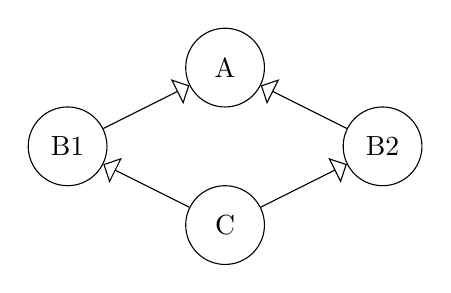
\begin{tikzpicture}[class/.style={draw,circle,minimum size=1cm},
                        inherits/.style={-{Triangle[open,length=5pt,width=10pt]}}]
      \node[class] (A) at (0,0) {A};
      \node[class] (B1) at (-2,-1) {B1};
      \node[class] (B2) at (2,-1) {B2};
      \node[class] (C) at (0,-2) {C};
      \draw[inherits] (B1) -- (A);
      \draw[inherits] (B2) -- (A);
      \draw[inherits] (C) -- (B1);
      \draw[inherits] (C) -- (B2);
    \end{tikzpicture}
  \end{center}
\end{frame}

\begin{frame}
  \frametitle{Problems With Multiple Inheritance}
  \code[font size=\small]{multiple-inheritance.cpp}
  \begin{itemize}
    \item {\tt C} inherits from {\tt A} twice
    \item $\rightarrow$ {\tt C} inherits {\tt x} twice!
    \item Each {\tt C} object has two {\tt x} variables
    \item Called \link{http://www.cprogramming.com/tutorial/virtual_inheritance.html}{Diamond Problem}
  \end{itemize}
\end{frame}

\begin{frame}
  \frametitle{Preventing Inheriting Member Variables Twice}
  \code[font size=\small]{virtual-inheritance-example.cpp}
  \begin{itemize}
    \item \link{https://en.wikipedia.org/wiki/Virtual_inheritance}{Virtual inheritance}
    \item {\tt A} is only inherited once by {\tt C}
    \item Has some weird consequences
    \item Generally discouraged
    \item Just know that it exists
  \end{itemize}
\end{frame}

\section{Other Details}

\begin{frame}
  \tableofcontents[currentsection]
\end{frame}

\begin{frame}
  \frametitle{Constructors}
  \begin{itemize}
    \item First thing a constructor must do is call superconstructor
    \item Akin to building a house: stories built from bottom to top
    \item Same as in Java
  \end{itemize}
  \code{constructors.cpp}
\end{frame}

\begin{frame}
  \frametitle{Stepwise Object Construction}
  \code{constructors2.cpp}
  \begin{center}
    \begin{tikzpicture}[layer/.style={draw,minimum width=5cm,minimum height=1cm}]
      \visible<2->{
        \node[layer] (A) at (0,0) {A};
      }

      \visible<3->{
        \node[layer,anchor=south west] (B) at (A.north west) {B};
      }

      \visible<4->{
        \node[layer,anchor=south west] (C) at (B.north west) {C};
      }

      \visible<handout:1|0>{
        \draw[-latex,thick] ($ (A.south west) + (-1,0) $) -- ($ (C.north west) + (-1, 0) $);
      }
    \end{tikzpicture}
  \end{center}
\end{frame}

\begin{frame}
  \frametitle{Calling Virtual Functions in Constructor}
  \begin{itemize}
    \item Just don't do it
  \end{itemize}
  \code[font size=\small]{virtual-calls.cpp}
\end{frame}

\begin{frame}
  \frametitle{Destructors}
  \begin{itemize}
    \item Last thing a destructor must do is call superdestructor
    \item Always happens automatically, no need to do it yourself
    \item Akin to destroying a house: stories removed from top to bottom
  \end{itemize}
\end{frame}

\begin{frame}
  \frametitle{Stepwise Object Destruction}
  \code{destructors.cpp}
  \begin{center}
    \begin{tikzpicture}[layer/.style={draw,minimum width=5cm,minimum height=1cm}]
      \visible<-3>{
        \node[layer] (A) at (0,0) {A};
      }

      \visible<-2>{
        \node[layer,anchor=south west] (B) at (A.north west) {B};
      }

      \visible<-1>{
        \node[layer,anchor=south west] (C) at (B.north west) {C};
      }

      \visible<handout:1|0>{
        \draw[-latex,thick] ($ (C.north west) + (-1, 0) $) -- ($ (A.south west) + (-1,0) $);
      }
    \end{tikzpicture}
  \end{center}
  \visible<4>{}
\end{frame}

\begin{frame}
  \frametitle{Destructors: Important}
  \code[font size=\small]{virtual-destructors.cpp}
\end{frame}

\begin{frame}
  \frametitle{Destructors: Important}
  \begin{itemize}
    \item {\tt delete} needs to know the dynamic type so as to
          call the correct destructor
    \item Destructor must be virtual
          \vskip2mm
          \code[font size=\small]{virtual-destructors2.cpp}
    \item Why not abstract? \cake
          \vskip2mm
          \code[font size=\small]{virtual-destructors3.cpp}
    \item Rule of thumb: add virtual destructor to each class
  \end{itemize}
\end{frame}

\end{document}


%%% Local Variables:
%%% mode: latex
%%% TeX-master: "inheritance"
%%% End:
